\chapter{Evaluation}
Give some introduction why you are doing these measurements.
Also an overview to allow the reader to find fast what he wants to read.

In general focus when describing on the why and implications.
Just putting plots there and describing is the easy part and does not give the reader insights beyond the plots.
You have to collect the clues and show what happens in the background to explain the development.

Here we evaluate different plotting frameworks to give you an alternative and show you some differences. This is continued in the discussion.

\section{Setup}
State the machines you are using the methods and the compiler if its system level.
Otherwise this section should tell all the steps necessary to reproduce your measurements.

Wollte eig nen barplot, lineplot und noch was mit log scale in allen dreien zeigen und jeweils was es speziell macht.


\section{Latency}
\begin{figure}
    \centering
    \subcaptionbox {Random write} {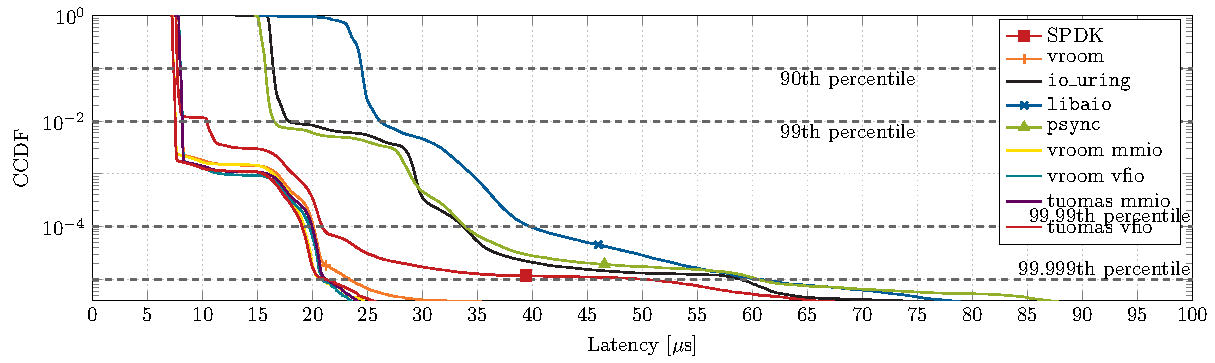
\includegraphics[width=\textwidth]{figures/latency-ccdf-write} \label{fig:ccdf-write}}
    \caption{Tail latencies}
    \label{fig:ccdf}
\end{figure}

\section{Matplotlib}

\section{ggplot}

\section{Seaborn}
